\documentclass[9pt,twoside,lineno]{pnas-new}
\usepackage{longtable}
\usepackage{tabularx}

\templatetype{pnassupportinginfo}
% Generated by scripts/build_paper_claim_ledger.py; do not edit by hand.
\providecommand{\PaperRoundingPolicy}{Four decimals for absolute metrics; two percentage points for development effects; three decimals for correlations and pair-level metrics.}
\providecommand{\AlignedMinusShiftedAUPRCLower}{0.1767}
\providecommand{\AlignedMinusShiftedAUPRCMedian}{0.1993}
\providecommand{\AlignedMinusShiftedAUPRCUpper}{0.2239}
\providecommand{\AlignedMinusShiftedAUROCLower}{0.1754}
\providecommand{\AlignedMinusShiftedAUROCMedian}{0.1926}
\providecommand{\AlignedMinusShiftedAUROCUpper}{0.2109}
\providecommand{\AlignedMinusShiftedFOneLower}{0.1155}
\providecommand{\AlignedMinusShiftedFOneMedian}{0.1311}
\providecommand{\AlignedMinusShiftedFOneUpper}{0.1477}
\providecommand{\AllADeltaAUPRCLower}{-0.0967}
\providecommand{\AllADeltaAUPRCMedian}{-0.0673}
\providecommand{\AllADeltaAUPRCUpper}{-0.0404}
\providecommand{\AllADeltaAUROCLower}{-0.0925}
\providecommand{\AllADeltaAUROCMedian}{-0.0664}
\providecommand{\AllADeltaAUROCUpper}{-0.0438}
\providecommand{\AllADeltaBrierLower}{0.0330}
\providecommand{\AllADeltaBrierMedian}{0.0497}
\providecommand{\AllADeltaBrierUpper}{0.0677}
\providecommand{\AllADeltaFOneLower}{-0.0878}
\providecommand{\AllADeltaFOneMedian}{-0.0599}
\providecommand{\AllADeltaFOneUpper}{-0.0365}
\providecommand{\ArteryADARProAUPRC}{0.9485}
\providecommand{\ArteryADARProAUROC}{0.9477}
\providecommand{\ArteryADARProBrier}{0.0879}
\providecommand{\ArteryADARProFOne}{0.8869}
\providecommand{\ArteryADARProPrecision}{0.8840}
\providecommand{\ArteryADARProRecall}{0.8899}
\providecommand{\ArteryADARProSpecificity}{0.8650}
\providecommand{\ArteryAdarEditAUPRC}{0.9262}
\providecommand{\ArteryAdarEditAUROC}{0.9238}
\providecommand{\ArteryAdarEditBrier}{0.1077}
\providecommand{\ArteryAdarEditFOne}{0.8671}
\providecommand{\ArteryAdarEditPrecision}{0.8345}
\providecommand{\ArteryAdarEditRecall}{0.9023}
\providecommand{\ArteryAdarEditSpecificity}{0.7930}
\providecommand{\ArteryDeltaAUPRC}{0.0224}
\providecommand{\ArteryDeltaAUROC}{0.0239}
\providecommand{\ArteryDeltaBrier}{-0.0198}
\providecommand{\ArteryDeltaFOne}{0.0199}
\providecommand{\ArteryDeltaPrecision}{0.0496}
\providecommand{\ArteryDeltaRecall}{-0.0125}
\providecommand{\ArteryDeltaSpecificity}{0.0720}
\providecommand{\ArteryEngagementCombinedGeometryAnyEditedAUROC}{0.816}
\providecommand{\ArteryEngagementCombinedGeometryRSquared}{0.270}
\providecommand{\ArteryEngagementCombinedGeometrySpearman}{0.536}
\providecommand{\ArteryEngagementGraphOnlyAnyEditedAUROC}{0.461}
\providecommand{\ArteryEngagementGraphOnlyRSquared}{0.053}
\providecommand{\ArteryEngagementGraphOnlySpearman}{0.203}
\providecommand{\ArteryFPRescueRate}{43.9}
\providecommand{\ArteryGapRho}{-0.482}
\providecommand{\ArteryMatchedRecallFPAvoided}{126}
\providecommand{\ArteryPairFirstAUPRCLower}{+0.79}
\providecommand{\ArteryPairFirstAUPRCMedian}{+1.37}
\providecommand{\ArteryPairFirstAUPRCUpper}{+1.97}
\providecommand{\ArteryPairFirstAUROCLower}{+0.80}
\providecommand{\ArteryPairFirstAUROCMedian}{+1.22}
\providecommand{\ArteryPairFirstAUROCUpper}{+1.66}
\providecommand{\ArteryPairFirstFOneLower}{+0.10}
\providecommand{\ArteryPairFirstFOneMedian}{+0.69}
\providecommand{\ArteryPairFirstFOneUpper}{+1.27}
\providecommand{\ArteryTPDamageRate}{4.9}
\providecommand{\BrainADARProAUPRC}{0.9504}
\providecommand{\BrainADARProAUROC}{0.9508}
\providecommand{\BrainADARProBrier}{0.0855}
\providecommand{\BrainADARProFOne}{0.8902}
\providecommand{\BrainADARProPrecision}{0.8741}
\providecommand{\BrainADARProRecall}{0.9069}
\providecommand{\BrainADARProSpecificity}{0.8529}
\providecommand{\BrainAdarEditAUPRC}{0.9286}
\providecommand{\BrainAdarEditAUROC}{0.9301}
\providecommand{\BrainAdarEditBrier}{0.1050}
\providecommand{\BrainAdarEditFOne}{0.8689}
\providecommand{\BrainAdarEditPrecision}{0.8371}
\providecommand{\BrainAdarEditRecall}{0.9032}
\providecommand{\BrainAdarEditSpecificity}{0.8021}
\providecommand{\BrainDeltaAUPRC}{0.0217}
\providecommand{\BrainDeltaAUROC}{0.0206}
\providecommand{\BrainDeltaBrier}{-0.0195}
\providecommand{\BrainDeltaFOne}{0.0213}
\providecommand{\BrainDeltaPrecision}{0.0370}
\providecommand{\BrainDeltaRecall}{0.0037}
\providecommand{\BrainDeltaSpecificity}{0.0507}
\providecommand{\BrainEngagementCombinedGeometryAnyEditedAUROC}{0.749}
\providecommand{\BrainEngagementCombinedGeometryRSquared}{0.239}
\providecommand{\BrainEngagementCombinedGeometrySpearman}{0.501}
\providecommand{\BrainEngagementGraphOnlyAnyEditedAUROC}{0.525}
\providecommand{\BrainEngagementGraphOnlyRSquared}{0.050}
\providecommand{\BrainEngagementGraphOnlySpearman}{0.218}
\providecommand{\BrainFPRescueRate}{38.6}
\providecommand{\BrainGapRho}{-0.425}
\providecommand{\BrainMatchedRecallFPAvoided}{119}
\providecommand{\BrainPairFirstAUPRCLower}{+1.02}
\providecommand{\BrainPairFirstAUPRCMedian}{+1.64}
\providecommand{\BrainPairFirstAUPRCUpper}{+2.20}
\providecommand{\BrainPairFirstAUROCLower}{+0.82}
\providecommand{\BrainPairFirstAUROCMedian}{+1.17}
\providecommand{\BrainPairFirstAUROCUpper}{+1.54}
\providecommand{\BrainPairFirstFOneLower}{+0.61}
\providecommand{\BrainPairFirstFOneMedian}{+1.11}
\providecommand{\BrainPairFirstFOneUpper}{+1.64}
\providecommand{\BrainTPDamageRate}{3.3}
\providecommand{\CombinedADARProAUPRC}{0.9513}
\providecommand{\CombinedADARProAUROC}{0.9491}
\providecommand{\CombinedADARProBrier}{0.0870}
\providecommand{\CombinedADARProFOne}{0.8852}
\providecommand{\CombinedADARProPrecision}{0.8463}
\providecommand{\CombinedADARProRecall}{0.9279}
\providecommand{\CombinedADARProSpecificity}{0.8159}
\providecommand{\CombinedAdarEditAUPRC}{0.9356}
\providecommand{\CombinedAdarEditAUROC}{0.9331}
\providecommand{\CombinedAdarEditBrier}{0.1043}
\providecommand{\CombinedAdarEditFOne}{0.8674}
\providecommand{\CombinedAdarEditPrecision}{0.8334}
\providecommand{\CombinedAdarEditRecall}{0.9043}
\providecommand{\CombinedAdarEditSpecificity}{0.8026}
\providecommand{\CombinedDeltaAUPRC}{0.0157}
\providecommand{\CombinedDeltaAUROC}{0.0160}
\providecommand{\CombinedDeltaBrier}{-0.0173}
\providecommand{\CombinedDeltaFOne}{0.0178}
\providecommand{\CombinedDeltaPrecision}{0.0129}
\providecommand{\CombinedDeltaRecall}{0.0236}
\providecommand{\CombinedDeltaSpecificity}{0.0133}
\providecommand{\CombinedFPRescueRate}{32.0}
\providecommand{\CombinedMatchedRecallFPAvoided}{148}
\providecommand{\CombinedPairFirstAUPRCLower}{+1.15}
\providecommand{\CombinedPairFirstAUPRCMedian}{+1.69}
\providecommand{\CombinedPairFirstAUPRCUpper}{+2.24}
\providecommand{\CombinedPairFirstAUROCLower}{+1.09}
\providecommand{\CombinedPairFirstAUROCMedian}{+1.45}
\providecommand{\CombinedPairFirstAUROCUpper}{+1.84}
\providecommand{\CombinedPairFirstFOneLower}{+0.94}
\providecommand{\CombinedPairFirstFOneMedian}{+1.41}
\providecommand{\CombinedPairFirstFOneUpper}{+1.98}
\providecommand{\CombinedTPDamageRate}{1.7}
\providecommand{\DevelopmentFoldSeed}{20260821}
\providecommand{\EngagementGateDeltaAUPRCLower}{0.0019}
\providecommand{\EngagementGateDeltaAUPRCMedian}{0.0084}
\providecommand{\EngagementGateDeltaAUPRCUpper}{0.0147}
\providecommand{\EngagementGateDeltaAUROCLower}{-0.0003}
\providecommand{\EngagementGateDeltaAUROCMedian}{0.0065}
\providecommand{\EngagementGateDeltaAUROCUpper}{0.0127}
\providecommand{\EngagementGateDeltaBrierLower}{-0.0028}
\providecommand{\EngagementGateDeltaBrierMedian}{0.0051}
\providecommand{\EngagementGateDeltaBrierUpper}{0.0126}
\providecommand{\EngagementGateDeltaFOneLower}{-0.0014}
\providecommand{\EngagementGateDeltaFOneMedian}{0.0041}
\providecommand{\EngagementGateDeltaFOneUpper}{0.0095}
\providecommand{\EnsembleComponentWeight}{0.5}
\providecommand{\EnsembleParameters}{80,138}
\providecommand{\FrozenEnsembleAUPRC}{0.9040}
\providecommand{\FrozenEnsembleAUROC}{0.9142}
\providecommand{\FrozenEnsembleBrier}{0.1168}
\providecommand{\FrozenEnsembleFOne}{0.8347}
\providecommand{\LiverADARProAUPRC}{0.9500}
\providecommand{\LiverADARProAUROC}{0.9414}
\providecommand{\LiverADARProBrier}{0.0951}
\providecommand{\LiverADARProFOne}{0.8812}
\providecommand{\LiverADARProPrecision}{0.8946}
\providecommand{\LiverADARProRecall}{0.8683}
\providecommand{\LiverADARProSpecificity}{0.8670}
\providecommand{\LiverAdarEditAUPRC}{0.9242}
\providecommand{\LiverAdarEditAUROC}{0.9092}
\providecommand{\LiverAdarEditBrier}{0.1196}
\providecommand{\LiverAdarEditFOne}{0.8541}
\providecommand{\LiverAdarEditPrecision}{0.8368}
\providecommand{\LiverAdarEditRecall}{0.8721}
\providecommand{\LiverAdarEditSpecificity}{0.7788}
\providecommand{\LiverDeltaAUPRC}{0.0258}
\providecommand{\LiverDeltaAUROC}{0.0322}
\providecommand{\LiverDeltaBrier}{-0.0245}
\providecommand{\LiverDeltaFOne}{0.0271}
\providecommand{\LiverDeltaPrecision}{0.0578}
\providecommand{\LiverDeltaRecall}{-0.0038}
\providecommand{\LiverDeltaSpecificity}{0.0881}
\providecommand{\LiverEngagementCombinedGeometryAnyEditedAUROC}{0.728}
\providecommand{\LiverEngagementCombinedGeometryRSquared}{0.277}
\providecommand{\LiverEngagementCombinedGeometrySpearman}{0.549}
\providecommand{\LiverEngagementGraphOnlyAnyEditedAUROC}{0.480}
\providecommand{\LiverEngagementGraphOnlyRSquared}{0.070}
\providecommand{\LiverEngagementGraphOnlySpearman}{0.246}
\providecommand{\LiverEnsembleDeltaAUPRCLower}{0.0171}
\providecommand{\LiverEnsembleDeltaAUPRCMedian}{0.0214}
\providecommand{\LiverEnsembleDeltaAUPRCUpper}{0.0263}
\providecommand{\LiverEnsembleDeltaAUROCLower}{0.0155}
\providecommand{\LiverEnsembleDeltaAUROCMedian}{0.0182}
\providecommand{\LiverEnsembleDeltaAUROCUpper}{0.0215}
\providecommand{\LiverEnsembleDeltaFOneLower}{0.0135}
\providecommand{\LiverEnsembleDeltaFOneMedian}{0.0179}
\providecommand{\LiverEnsembleDeltaFOneUpper}{0.0225}
\providecommand{\LiverFPRescueRate}{50.6}
\providecommand{\LiverGapRho}{-0.475}
\providecommand{\LiverMatchedRecallFPAvoided}{158}
\providecommand{\LiverPairFirstAUPRCLower}{+0.70}
\providecommand{\LiverPairFirstAUPRCMedian}{+1.72}
\providecommand{\LiverPairFirstAUPRCUpper}{+2.71}
\providecommand{\LiverPairFirstAUROCLower}{+1.18}
\providecommand{\LiverPairFirstAUROCMedian}{+1.79}
\providecommand{\LiverPairFirstAUROCUpper}{+2.37}
\providecommand{\LiverPairFirstFOneLower}{+0.96}
\providecommand{\LiverPairFirstFOneMedian}{+1.64}
\providecommand{\LiverPairFirstFOneUpper}{+2.30}
\providecommand{\LiverTPDamageRate}{5.9}
\providecommand{\LocalControlShift}{96}
\providecommand{\LocalWindowWidth}{65}
\providecommand{\MacroDeltaAUPRC}{0.0261}
\providecommand{\MacroDeltaAUROC}{0.0277}
\providecommand{\MacroDeltaBrier}{-0.0208}
\providecommand{\MacroDeltaFOne}{0.0253}
\providecommand{\MacroDeltaPrecision}{0.0407}
\providecommand{\MacroDeltaRecall}{0.0087}
\providecommand{\MacroDeltaSpecificity}{0.0576}
\providecommand{\MultitaskDeltaAUPRCLower}{-0.0010}
\providecommand{\MultitaskDeltaAUPRCMedian}{0.0087}
\providecommand{\MultitaskDeltaAUPRCUpper}{0.0179}
\providecommand{\MultitaskDeltaAUROCLower}{0.0010}
\providecommand{\MultitaskDeltaAUROCMedian}{0.0081}
\providecommand{\MultitaskDeltaAUROCUpper}{0.0151}
\providecommand{\MultitaskDeltaBrierLower}{-0.0122}
\providecommand{\MultitaskDeltaBrierMedian}{-0.0069}
\providecommand{\MultitaskDeltaBrierUpper}{-0.0011}
\providecommand{\MultitaskDeltaFOneLower}{-0.0071}
\providecommand{\MultitaskDeltaFOneMedian}{0.0008}
\providecommand{\MultitaskDeltaFOneUpper}{0.0086}
\providecommand{\MuscleADARProAUPRC}{0.9207}
\providecommand{\MuscleADARProAUROC}{0.9144}
\providecommand{\MuscleADARProBrier}{0.1296}
\providecommand{\MuscleADARProFOne}{0.8541}
\providecommand{\MuscleADARProPrecision}{0.8230}
\providecommand{\MuscleADARProRecall}{0.8876}
\providecommand{\MuscleADARProSpecificity}{0.7788}
\providecommand{\MuscleAdarEditAUPRC}{0.8757}
\providecommand{\MuscleAdarEditAUROC}{0.8688}
\providecommand{\MuscleAdarEditBrier}{0.1526}
\providecommand{\MuscleAdarEditFOne}{0.8139}
\providecommand{\MuscleAdarEditPrecision}{0.7767}
\providecommand{\MuscleAdarEditRecall}{0.8549}
\providecommand{\MuscleAdarEditSpecificity}{0.7152}
\providecommand{\MuscleDeltaAUPRC}{0.0450}
\providecommand{\MuscleDeltaAUROC}{0.0456}
\providecommand{\MuscleDeltaBrier}{-0.0230}
\providecommand{\MuscleDeltaFOne}{0.0401}
\providecommand{\MuscleDeltaPrecision}{0.0463}
\providecommand{\MuscleDeltaRecall}{0.0327}
\providecommand{\MuscleDeltaSpecificity}{0.0636}
\providecommand{\MuscleEngagementCombinedGeometryAnyEditedAUROC}{0.705}
\providecommand{\MuscleEngagementCombinedGeometryRSquared}{0.050}
\providecommand{\MuscleEngagementCombinedGeometrySpearman}{0.322}
\providecommand{\MuscleEngagementGraphOnlyAnyEditedAUROC}{0.557}
\providecommand{\MuscleEngagementGraphOnlyRSquared}{0.010}
\providecommand{\MuscleEngagementGraphOnlySpearman}{0.123}
\providecommand{\MuscleEnsembleDeltaAUPRCLower}{0.0236}
\providecommand{\MuscleEnsembleDeltaAUPRCMedian}{0.0308}
\providecommand{\MuscleEnsembleDeltaAUPRCUpper}{0.0384}
\providecommand{\MuscleEnsembleDeltaAUROCLower}{0.0207}
\providecommand{\MuscleEnsembleDeltaAUROCMedian}{0.0256}
\providecommand{\MuscleEnsembleDeltaAUROCUpper}{0.0305}
\providecommand{\MuscleEnsembleDeltaFOneLower}{0.0045}
\providecommand{\MuscleEnsembleDeltaFOneMedian}{0.0139}
\providecommand{\MuscleEnsembleDeltaFOneUpper}{0.0234}
\providecommand{\MuscleExpandedSiteAUPRC}{0.8520}
\providecommand{\MuscleExpandedSiteAUROC}{0.8659}
\providecommand{\MuscleExpandedSiteBrier}{0.1515}
\providecommand{\MuscleExpandedSiteFOne}{0.7924}
\providecommand{\MuscleFPRescueRate}{44.1}
\providecommand{\MuscleGapRho}{-0.334}
\providecommand{\MuscleInternalReferenceAUPRC}{0.8256}
\providecommand{\MuscleInternalReferenceAUROC}{0.8456}
\providecommand{\MuscleInternalReferenceBrier}{0.1695}
\providecommand{\MuscleInternalReferenceFOne}{0.7783}
\providecommand{\MuscleLabelExpansionAUPRCLower}{+1.25}
\providecommand{\MuscleLabelExpansionAUPRCMedian}{+2.63}
\providecommand{\MuscleLabelExpansionAUPRCUpper}{+4.17}
\providecommand{\MuscleLabelExpansionAUROCLower}{+1.06}
\providecommand{\MuscleLabelExpansionAUROCMedian}{+2.04}
\providecommand{\MuscleLabelExpansionAUROCUpper}{+3.00}
\providecommand{\MuscleLabelExpansionBrierLower}{-2.46}
\providecommand{\MuscleLabelExpansionBrierMedian}{-1.80}
\providecommand{\MuscleLabelExpansionBrierUpper}{-1.10}
\providecommand{\MuscleLabelExpansionFOneLower}{+0.21}
\providecommand{\MuscleLabelExpansionFOneMedian}{+1.42}
\providecommand{\MuscleLabelExpansionFOneUpper}{+2.57}
\providecommand{\MuscleLocalAUPRC}{0.8936}
\providecommand{\MuscleLocalAUROC}{0.9045}
\providecommand{\MuscleLocalFOne}{0.8337}
\providecommand{\MuscleMatchedRecallFPAvoided}{68}
\providecommand{\MusclePairAUPRC}{0.8730}
\providecommand{\MusclePairAUROC}{0.8885}
\providecommand{\MusclePairFOne}{0.8208}
\providecommand{\MusclePairFirstAUPRC}{0.8730}
\providecommand{\MusclePairFirstAUPRCLower}{+3.15}
\providecommand{\MusclePairFirstAUPRCMedian}{+4.73}
\providecommand{\MusclePairFirstAUPRCUpper}{+6.35}
\providecommand{\MusclePairFirstAUROC}{0.8885}
\providecommand{\MusclePairFirstAUROCLower}{+3.07}
\providecommand{\MusclePairFirstAUROCMedian}{+4.28}
\providecommand{\MusclePairFirstAUROCUpper}{+5.49}
\providecommand{\MusclePairFirstBrier}{0.1372}
\providecommand{\MusclePairFirstFOne}{0.8208}
\providecommand{\MusclePairFirstFOneLower}{+3.11}
\providecommand{\MusclePairFirstFOneMedian}{+4.23}
\providecommand{\MusclePairFirstFOneUpper}{+5.38}
\providecommand{\MusclePairFirstIncrementAUPRCLower}{+0.76}
\providecommand{\MusclePairFirstIncrementAUPRCMedian}{+2.08}
\providecommand{\MusclePairFirstIncrementAUPRCUpper}{+3.55}
\providecommand{\MusclePairFirstIncrementAUROCLower}{+1.25}
\providecommand{\MusclePairFirstIncrementAUROCMedian}{+2.27}
\providecommand{\MusclePairFirstIncrementAUROCUpper}{+3.36}
\providecommand{\MusclePairFirstIncrementBrierLower}{-2.24}
\providecommand{\MusclePairFirstIncrementBrierMedian}{-1.45}
\providecommand{\MusclePairFirstIncrementBrierUpper}{-0.71}
\providecommand{\MusclePairFirstIncrementFOneLower}{+1.68}
\providecommand{\MusclePairFirstIncrementFOneMedian}{+2.85}
\providecommand{\MusclePairFirstIncrementFOneUpper}{+4.01}
\providecommand{\MusclePairFirstTotalAUPRCLower}{+3.34}
\providecommand{\MusclePairFirstTotalAUPRCMedian}{+4.73}
\providecommand{\MusclePairFirstTotalAUPRCUpper}{+6.30}
\providecommand{\MusclePairFirstTotalAUROCLower}{+3.19}
\providecommand{\MusclePairFirstTotalAUROCMedian}{+4.29}
\providecommand{\MusclePairFirstTotalAUROCUpper}{+5.50}
\providecommand{\MusclePairFirstTotalBrierLower}{-4.11}
\providecommand{\MusclePairFirstTotalBrierMedian}{-3.24}
\providecommand{\MusclePairFirstTotalBrierUpper}{-2.45}
\providecommand{\MusclePairFirstTotalFOneLower}{+3.16}
\providecommand{\MusclePairFirstTotalFOneMedian}{+4.26}
\providecommand{\MusclePairFirstTotalFOneUpper}{+5.39}
\providecommand{\MuscleShiftedAUPRC}{0.6943}
\providecommand{\MuscleShiftedAUROC}{0.7122}
\providecommand{\MuscleShiftedFOne}{0.7028}
\providecommand{\MuscleTPDamageRate}{4.3}
\providecommand{\NBootstrapReplicates}{2,000}
\providecommand{\NCanonicalEvaluations}{1}
\providecommand{\NFinalComponentFits}{10}
\providecommand{\NOuterFolds}{5}
\providecommand{\NSubstrates}{884}
\providecommand{\NTestPairs}{179}
\providecommand{\NTrainPairs}{566}
\providecommand{\NValidationPairs}{139}
\providecommand{\NegativeThresholdPct}{1}
\providecommand{\PositiveThresholdPct}{15}
\providecommand{\PretrainingCandidatePairs}{288,056}
\providecommand{\SharedMacroDeltaAUPRCLower}{0.0075}
\providecommand{\SharedMacroDeltaAUPRCMedian}{0.0114}
\providecommand{\SharedMacroDeltaAUPRCUpper}{0.0157}
\providecommand{\SharedMacroDeltaAUROCLower}{0.0058}
\providecommand{\SharedMacroDeltaAUROCMedian}{0.0087}
\providecommand{\SharedMacroDeltaAUROCUpper}{0.0115}
\providecommand{\SharedMacroDeltaBrierLower}{-0.0005}
\providecommand{\SharedMacroDeltaBrierMedian}{0.0043}
\providecommand{\SharedMacroDeltaBrierUpper}{0.0092}
\providecommand{\SharedMacroDeltaFOneLower}{0.0037}
\providecommand{\SharedMacroDeltaFOneMedian}{0.0075}
\providecommand{\SharedMacroDeltaFOneUpper}{0.0113}
\providecommand{\UnifiedAUPRC}{0.8922}
\providecommand{\UnifiedAUROC}{0.9072}
\providecommand{\UnifiedAuxWeight}{0.25}
\providecommand{\UnifiedBaseSeed}{20,260,821}
\providecommand{\UnifiedBatchSize}{256}
\providecommand{\UnifiedBrier}{0.1372}
\providecommand{\UnifiedDeltaAUPRCLower}{-0.0202}
\providecommand{\UnifiedDeltaAUPRCMedian}{-0.0118}
\providecommand{\UnifiedDeltaAUPRCUpper}{-0.0043}
\providecommand{\UnifiedDeltaAUROCLower}{-0.0129}
\providecommand{\UnifiedDeltaAUROCMedian}{-0.0072}
\providecommand{\UnifiedDeltaAUROCUpper}{-0.0015}
\providecommand{\UnifiedDeltaBrierLower}{0.0135}
\providecommand{\UnifiedDeltaBrierMedian}{0.0205}
\providecommand{\UnifiedDeltaBrierUpper}{0.0276}
\providecommand{\UnifiedDeltaFOneLower}{-0.0125}
\providecommand{\UnifiedDeltaFOneMedian}{-0.0030}
\providecommand{\UnifiedDeltaFOneUpper}{0.0066}
\providecommand{\UnifiedEpochs}{1,000}
\providecommand{\UnifiedFOne}{0.8317}
\providecommand{\UnifiedPairs}{585}
\providecommand{\UnifiedParameters}{65,698}
\providecommand{\UnifiedRows}{5,967}


% Compatibility shim for the current PNAS class/SI-style combination.
\makeatletter
\@ifundefined{PNAS@linecount}{\newcount\PNAS@linecount\PNAS@linecount\@ne}{}
\makeatother

\title{Supporting Information for: Systematic dissection of endogenous A-to-I RNA editing reveals substrate- and target-level determinants of predictability}
\author{Author list pending}
\correspondingauthor{Corresponding author and e-mail pending author confirmation.}

\begin{document}

\maketitle
\SItext

This appendix provides the complete scientific argument behind the ADARPro campaign, including branches that were limited, stopped, or deferred. Four evidence categories remain distinct throughout: \emph{development OOF} denotes pair-disjoint cross-fitted comparisons used for discovery and selection; \emph{selection diagnostic} denotes published-validation quantities used for checkpoints or thresholds; \emph{canonical held-out} denotes the single evaluation after the final manifest was frozen; and \emph{secondary} denotes robustness or descriptive analyses that do not define the benchmark claim. ``Not supported'' always means not supported by the tested representation at the available resolution. A deferred hypothesis lacked a benchmark-compatible measurement and was not counted as negative evidence.

\section*{A. Benchmark reproduction and leakage control}

\subsection*{Immutable AdarEdit benchmark}

The upstream AdarEdit reproducibility release was preserved at the immutable revision recorded in repository provenance. Environment, package, GPU, input-file, and checkpoint provenance are retained in the repository. The upstream verifier recovered \NSubstrates{} graph-buildable inverted-Alu pairs: \NTrainPairs{} train, \NValidationPairs{} validation, and \NTestPairs{} test, with no pair shared between partitions. Supplied Baseline GAT checkpoints reproduced the reported metrics for artery tibial, brain/cerebellum, liver, skeletal muscle, and Combined. Combined pools evidence across GTEx tissues and was never treated as a fifth tissue when constructing environmental covariates.

Each example contains both Alu arms in transcript orientation, a focal adenosine, predicted dot-bracket structure, and EditingIndex-derived label. EditingIndex $\geq\PositiveThresholdPct{}\%$ defines edited sites, EditingIndex $<\NegativeThresholdPct{}\%$ defines nonedited sites, and the canonical binary task excludes the intermediate interval. Nodes encode nucleotide and structure-derived features; edges represent backbone and predicted base-pair relations. The original construction used ViennaRNA for secondary structure \cite{Lorenz2011}.

\subsection*{Coordinates and authoritative observations}

Genomic coordinates were reconstructed with the original strand-aware transformation from local model positions to \textit{hg38}/GRCh38. Pair intervals came from \texttt{Pair\_Alu\_withStrand.bed}; raw tissue tables supplied focal positions and EditingIndex. Both \texttt{site\_id = chromosome:position:strand} and \texttt{(pair\_id, local\_position)} were retained. Quality control required an adenosine in transcript orientation, deterministic row mapping, correct strand, and stable identity across tissues. The resulting \texttt{site\_master.parquet} records labels, continuous editing values, sequence, structure, coordinates, folds, OOF predictions, and provenance.

\subsection*{Test quarantine, grouped folds, and inference}

Canonical test paths and SHA-256 values were registered before development. The quarantine library denied protected-path access unless a single-use authorization matched the frozen manifest. Discovery used the union of published train and validation pairs divided deterministically into \NOuterFolds{} outer folds by pair ID. Preprocessing, feature selection, dimensionality reduction, fitted residual models, checkpoints, and thresholds excluded the outer fold. A row entered an OOF table only after a model that had not seen its pair scored it.

The grouped OOF reference is an internal research instrument, not a revision of the published benchmark. Each outer model sees fewer pairs than a final fit and therefore has lower absolute performance. OOF comparisons estimate incremental value because candidate and reference share folds, training scope, and evaluation logic. The supplied-checkpoint canonical comparison answers the final benchmark question (Fig.~\ref{fig:s1}). Development differences are never added arithmetically to published test scores.

We report AUROC, AUPRC, F1, precision, recall, specificity, balanced accuracy, Matthews correlation coefficient, and Brier score. Unless specified otherwise, thresholds maximized F1 on fold-internal validation data. Paired confidence intervals use \NBootstrapReplicates{} bootstrap replicates sampling pair IDs with replacement and retaining every site from a sampled pair. Effect size and clustered uncertainty, rather than site-wise $P$ values, determine interpretation.

\begin{figure}[H]
\centering
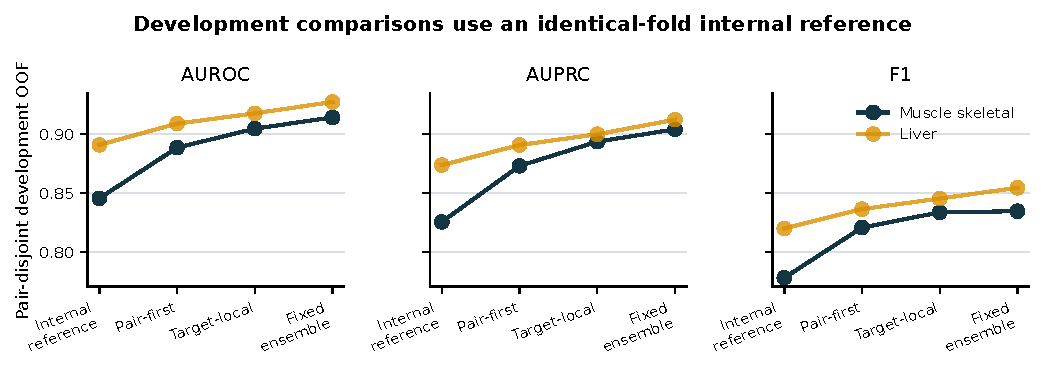
\includegraphics[width=\textwidth]{figures/figureS1_development_regime.pdf}
\caption{\textbf{Two evaluation regimes answer different questions.} Development OOF comparisons use an identical-fold internal reference to attribute incremental effects. The separately reproduced supplied-checkpoint canonical test is the authoritative final benchmark.}
\label{fig:s1}
\end{figure}

\begin{table}[H]
\centering
\caption{Complete one-use canonical held-out metrics. Thresholds were frozen from the published validation partition before test access. Combined is a pooled endpoint.}\label{tab:lockedmetrics}
\resizebox{\textwidth}{!}{%
\begin{tabular}{llrrrrrrr}
\toprule
Context & Model & AUROC & AUPRC & F1 & Precision & Recall & Specificity & Brier \\
\midrule
Artery & AdarEdit & 0.9238 & 0.9262 & 0.8671 & 0.8345 & 0.9023 & 0.7930 & 0.1077 \\
Artery & Selected predictor & 0.9477 & 0.9485 & 0.8869 & 0.8840 & 0.8899 & 0.8650 & 0.0879 \\
Brain & AdarEdit & 0.9301 & 0.9286 & 0.8689 & 0.8371 & 0.9032 & 0.8021 & 0.1050 \\
Brain & Selected predictor & 0.9508 & 0.9504 & 0.8902 & 0.8741 & 0.9069 & 0.8529 & 0.0855 \\
Liver & AdarEdit & 0.9092 & 0.9242 & 0.8541 & 0.8368 & 0.8721 & 0.7788 & 0.1196 \\
Liver & Selected predictor & 0.9414 & 0.9500 & 0.8812 & 0.8946 & 0.8683 & 0.8670 & 0.0951 \\
Skeletal muscle & AdarEdit & 0.8688 & 0.8757 & 0.8139 & 0.7767 & 0.8549 & 0.7152 & 0.1526 \\
Skeletal muscle & Selected predictor & 0.9144 & 0.9207 & 0.8541 & 0.8230 & 0.8876 & 0.7788 & 0.1296 \\
Combined & AdarEdit & 0.9331 & 0.9356 & 0.8674 & 0.8334 & 0.9043 & 0.8026 & 0.1043 \\
Combined & Selected predictor & 0.9491 & 0.9513 & 0.8852 & 0.8463 & 0.9279 & 0.8159 & 0.0870 \\
\bottomrule
\end{tabular}}
\end{table}


\section*{B. Complete hypothesis map}

The research tree was ranked before expensive model development by mechanistic rationale, novelty relative to AdarEdit, data compatibility, leakage risk, effective sample size, and expected performance upside. Directions advanced only after comparison with the appropriate same-fold reference and negative controls. The resulting taxonomy separates selected contributions, limited evidence, unsupported tested formulations, and hypotheses deferred because the required measurement was unavailable (Table~\ref{tab:evidencemap}). The complete machine-readable tree records each hypothesis, source, promotion rule, kill rule, and final decision; Table~\ref{tab:taxonomy} preserves the chronological disposition without turning run counts into a scientific result.

\begin{table}[p]
\centering
\caption{Development evidence map. Values are percentage-point changes in AUROC with 95\% whole-pair bootstrap intervals. Each row uses its preregistered or documented same-fold comparator; these heterogeneous estimands are an evidence synthesis, not a ranking of effect sizes.}\label{tab:evidencemap}
\resizebox{\textwidth}{!}{%
\begin{tabular}{llll}
\toprule
Axis & Hypothesis & Decision & $\Delta$AUROC [95\% CI] \\
\midrule
Supervision & Pair-first expanded supervision & Selected & +4.29 [+3.19, +5.50] \\
Representation & Target-aligned local view & Selected & +1.61 [+0.80, +2.38] \\
Integration & Fixed global + local ensemble & Selected & +2.56 [+2.07, +3.05] \\
Integration & Shared four-tissue training & Limited & +0.87 [+0.58, +1.15] \\
Supervision & Continuous/ordinal auxiliary loss & Limited & +0.81 [+0.10, +1.51] \\
Biology × AI & Substrate-engagement gate & Limited & +0.65 [-0.03, +1.27] \\
Biology & IRAlu/transcript architecture & Not Promoted & +0.16 [-0.79, +1.05] \\
Biology & H3K36me3 peak overlap & Not Promoted & +0.19 [-0.10, +0.47] \\
Biology & RBP suppressor panel & Not Promoted & -0.26 [-0.74, +0.26] \\
Representation & RiNALMo target embedding & Not Promoted & -0.05 [-0.51, +0.39] \\
Representation & Substrate-wide all-A decoder & Terminated & -6.64 [-9.25, -4.38] \\
Integration & Unified end-to-end model & Terminated & -0.72 [-1.29, -0.15] \\
\bottomrule
\end{tabular}}
\end{table}


\section*{C. Biological-context tests}

\subsection*{RBP occupancy, binding potential, and abundance}

Candidate RBPs were prioritized independently from model outcome using known ADAR interaction, dsRNA binding, perturbation evidence, nuclear localization, Alu association, expression, and assay availability. Experimental occupancy used replicated or high-confidence ENCODE eCLIP peaks \cite{VanNostrand2020}; predicted occupancy used PrismNet and RBPNet where compatible \cite{Sun2021PrismNet,Horlacher2023RBPNet}. Features included focal overlap, distance to the nearest peak, local-window signal, duplex-wide burden, arm asymmetry, partner occupancy, and regulator-class aggregates. GTEx medians supplied tissue abundance and binding-by-abundance interactions \cite{GTEx2020}. Combined received no artificial tissue vector.

Controls included randomized RBP identities, shuffled tissue vectors, matched-dimensional noise, abundance without binding, and binding without abundance. High-confidence baseline false positives were matched on baseline probability, tissue, structural state, and pair characteristics. None of the experimental-occupancy, predicted-binding, abundance, or interaction panels produced a reproducible residual increment beyond its controls (Fig.~\ref{fig:s2}). This operationalization is limited by cell-line/tissue mismatch and repeat mapping; absence of an eCLIP peak in Alu sequence was never interpreted as biological absence.

Label-switching sites hold sequence and predicted structure constant across individual tissues. In the available four-tissue comparison, tissue identity nearly separated switch direction by itself, so tissue-average expression could not establish a regulator-specific transferable mechanism. The branch was terminated rather than enlarged. Established RBP regulation of editing remains biologically compatible with this predictive result \cite{Freund2020,QuinonesValdez2019,Park2026,Yi2026}.

\subsection*{Transcript, repeat, and chromatin annotations}

Reconstructed pair intervals supplied arm separation and length, orientation, repeat subfamily and divergence, Alu-neighborhood composition, transcript overlap, and exon/intron annotations. Fold-isolated residual models combined standardized features with the baseline logit. The broad site-level panel did not generalize beyond the structure graph; this did not preclude a pair-level role for geometry (Section D).

Exact-tissue compatible H3K36me3 tracks were summarized at the target, local windows, arms, and entire pair. A chromosome-shifted overlap acted as a spatial control. H3K36me3 produced a weak liver AUPRC effect but no stable AUROC, F1, or engagement improvement (Fig.~\ref{fig:s2}). H2A.Z was not promoted to a benchmark experiment because no adequately matched and powered tissue resource was available. The result concerns information in bulk peak overlap, not chromatin causality \cite{Cai2026,ENCODE2020}.

\begin{figure}[H]
\centering
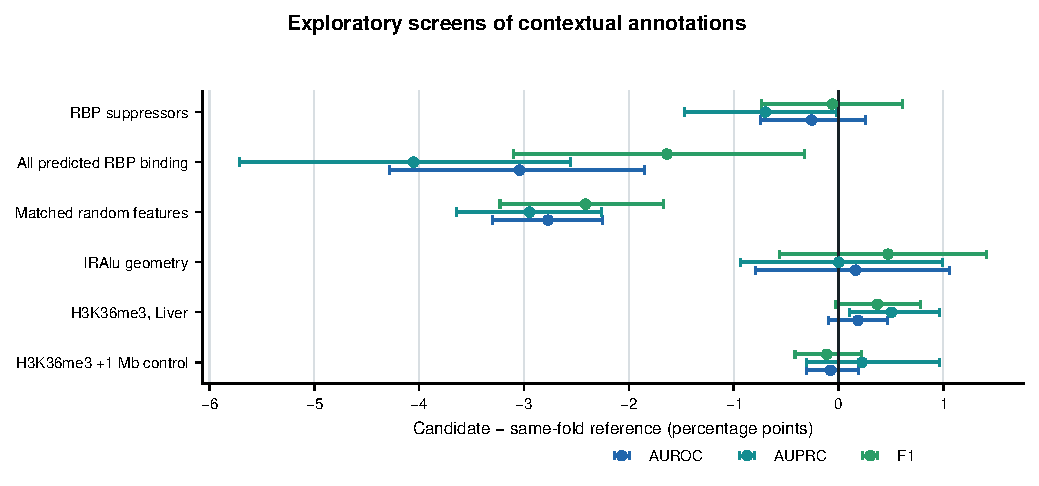
\includegraphics[width=\textwidth]{figures/figureS2_biological_feature_controls.pdf}
\caption{\textbf{Bulk biological annotations and matched controls.} Every point is labeled by formulation. Pair-bootstrap development differences use the documented same-fold reference. The RBP, genomic, and chromatin measurements shown did not add a reproducible increment across ranking and thresholded metrics.}
\label{fig:s2}
\end{figure}

\section*{D. Substrate realization}

Pair-level analyses used one row per development substrate. Outcomes were edited-site fraction, mean EditingIndex, and whether a pair contained any high-editing site. Predictors ranged from adenosine count and graph-derived sequence/structure summaries to genomic geometry and the combined 16-feature low-capacity model. All fitting remained inside pair folds.

Inter-arm gap correlated negatively with edited-site fraction in every individual tissue. Geometry plus graph summaries improved $R^2$ over graph summaries alone in all four tissues, with positive pair-bootstrap intervals (Table~\ref{tab:substraterealization}). The combined model also classified whether a pair contained any high-editing site above chance. These are direct observations that substrates differ in realized burden; they do not identify the cellular mechanism that realizes a duplex.

Site-level translation was weaker. Multiplying or gating site probabilities with cross-fitted engagement estimates increased AUPRC modestly but did not yield a stable F1 gain and worsened Brier score. A neural auxiliary engagement objective decreased the principal classification metric and was stopped. Static pair attributes can therefore describe realization propensity without recovering the time-, isoform-, transcript-, or cell-specific state required to alter the strongest site predictions.

\begin{table}[H]
\centering
\caption{\textbf{Genomic geometry improves prediction of the edited-site fraction in all four tissues.} Larger inter-arm gaps correlate with lower burden (Spearman $\rho$). Burden is the high-editing fraction among eligible high/low sites within a pair. Adding geometry to graph-derived summaries improves pair-level $R^2$; $\Delta R^2$ is relative to graph summaries alone, with a 95\% pair-clustered bootstrap interval. ``Any high'' asks whether a pair contains at least one site with EditingIndex $\geq15\%$. These outcomes measure editing burden, not molecular realization or ADAR engagement.}\label{tab:substraterealization}
\begin{tabular}{lrrrrr}
\toprule
Context & Gap--burden $\rho$ & Graph-only $R^2$ & Combined $R^2$ & $\Delta R^2$ [95\% CI], points & Any-high AUROC \\
\midrule
Artery & -0.482 & 0.053 & 0.270 & +21.64 [+16.39, +26.93] & 0.816 \\
Brain & -0.425 & 0.050 & 0.239 & +19.11 [+13.94, +23.68] & 0.749 \\
Liver & -0.475 & 0.070 & 0.277 & +20.82 [+15.75, +26.03] & 0.728 \\
Skeletal muscle & -0.334 & 0.010 & 0.050 & +4.12 [+0.99, +6.98] & 0.705 \\
\bottomrule
\end{tabular}
\end{table}


\section*{E. Richer supervision and the statistical unit}

The expanded training pool contains all eligible high- and low-editing observations in each training pair. The site-balanced formulation draws uniformly from those rows. The pair-first formulation draws a pair uniformly, a class with probability 0.5, and then an eligible site of that class; if the pair lacks that class, its available class is used. The canonical-row epoch budget was held fixed, preventing extra optimizer steps from explaining the difference.

The existing same-fold sequence original reference $\rightarrow$ expanded site-balanced $\rightarrow$ expanded pair-first separates the two corrections (Table~\ref{tab:supervisiondecomposition}). Label recovery improved all three primary metrics. With the label pool held constant, pair-first weighting added a second favorable increment, including \MusclePairFirstIncrementFOneMedian{} F1 points. Pair-first gains replicated across all endpoints (Table~\ref{tab:pairbalance}). This supports the pair as the unit of statistical dependence, without asserting that every site within a pair has identical biology.

The binary/ordinal/continuous model shared an encoder across canonical classification, ordinal bins, and transformed EditingIndex regression. It added a small ranking and Brier improvement over pair-balanced binary training, but essentially no F1. Adding it to the selected predictor reduced natural-prevalence F1, so the graded-label branch remained limited. Intermediate values contain ordering information, but they did not improve the primary thresholded task enough to justify added complexity.

\begin{table}[H]
\centering
\caption{\textbf{More valid labels and more balanced substrate weights make separate contributions.} In muscle development data, recovering eligible high/low labels improves prediction under row-wise sampling. Pair-first weighting adds a further gain with the label pool and class balance fixed. The same-fold comparisons isolate the label and weighting effects; intervals are pair-clustered bootstrap intervals for each indicated step, in percentage points.}\label{tab:supervisiondecomposition}
\begin{tabular}{lrrr@{\hspace{2\tabcolsep}\hspace{0.6em}}rr}
\toprule
Metric & Original reference & All high/low, row-wise & $\Delta$ from labels [95\% CI] & All high/low, pair-first & $\Delta$ from pair weighting [95\% CI] \\
\midrule
AUROC & 0.8456 & 0.8659 & +2.04 [+1.06, +3.00] & 0.8885 & +2.27 [+1.25, +3.36] \\
AUPRC & 0.8256 & 0.8520 & +2.63 [+1.25, +4.17] & 0.8730 & +2.08 [+0.76, +3.55] \\
F1 & 0.7783 & 0.7924 & +1.42 [+0.21, +2.57] & 0.8208 & +2.85 [+1.68, +4.01] \\
\bottomrule
\end{tabular}
\end{table}

\begin{table}[H]
\centering
\caption{\textbf{Expanded pair-first learning improves ranking and classification across all five endpoints.} The combined change in label coverage and within-class pair weighting outperforms the same-fold internal AdarEdit reference; every interval is positive. Values are percentage-point median differences with 95\% pair-clustered bootstrap intervals. Combined is pooled, and these development comparisons do not isolate weighting from label recovery outside muscle.}\label{tab:pairbalance}
\resizebox{\textwidth}{!}{%
\begin{tabular}{lrrr}
\toprule
Context & $\Delta$AUROC [95\% CI] & $\Delta$AUPRC [95\% CI] & $\Delta$F1 [95\% CI] \\
\midrule
Artery & +1.22 [+0.80, +1.66] & +1.37 [+0.79, +1.97] & +0.69 [+0.10, +1.27] \\
Brain & +1.17 [+0.82, +1.54] & +1.64 [+1.02, +2.20] & +1.11 [+0.61, +1.64] \\
Liver & +1.79 [+1.18, +2.37] & +1.72 [+0.70, +2.71] & +1.64 [+0.96, +2.30] \\
Skeletal muscle & +4.28 [+3.07, +5.49] & +4.73 [+3.15, +6.35] & +4.23 [+3.11, +5.38] \\
Combined & +1.45 [+1.09, +1.84] & +1.69 [+1.15, +2.24] & +1.41 [+0.94, +1.98] \\
\bottomrule
\end{tabular}}
\end{table}


\section*{F. Focal and target-local representation}

Three stages tested whether whole-duplex mean pooling loses site identity. First, fold-isolated target-contact geometry added AUROC and AUPRC but little F1, localizing a ranking effect near the target. Second, a focal-node graph model preserved the final target embedding alongside the global mean. It improved ranking relative to the pair model and an otherwise matched duplicate-global control, although its standalone F1 interval was insufficient for promotion. Third, the selected \LocalWindowWidth{}-position encoder aligned the focal adenosine with its dot-bracket partner and encoded nucleotide, pairing, validity, target/partner indicators, and relative position through two dilated convolutional layers.

The aligned local model exceeded the whole-duplex pair model in muscle and replicated in liver. Its matched-capacity control moved the same local window \LocalControlShift{} nt away while retaining all dimensions and optimization. The shifted model collapsed across AUROC, AUPRC, and F1 (Table~\ref{tab:targetcontrols}), demonstrating that alignment rather than generic convolutional capacity carries the improvement. Natural-prevalence results preserved the advantage (Fig.~\ref{fig:s3}).

\begin{table}[H]
\centering
\caption{\textbf{The aligned local window adds signal; shifting it loses the gain despite matched model capacity.} Explicit target retention improves on whole-duplex pooling, and the aligned graph-plus-local model improves further. Moving the local window while preserving the architecture reduces ranking and F1 and increases Brier error. This control tests target-centered neighborhood information, not partner identity alone. All values use the same canonical muscle development rows and out-of-fold predictions.}\label{tab:targetcontrols}
\begin{tabular}{lrrrr}
\toprule
Representation & AUROC & AUPRC & F1 & Brier \\
\midrule
Whole-duplex pair model & 0.8885 & 0.8730 & 0.8208 & 0.1372 \\
Explicit focal node & 0.9014 & 0.8902 & 0.8251 & 0.1342 \\
Graph + aligned target/helix-partner & 0.9045 & 0.8936 & 0.8337 & 0.1286 \\
Matched-capacity +96-nt shift & 0.7122 & 0.6943 & 0.7028 & 0.2356 \\
\bottomrule
\end{tabular}
\end{table}


\section*{G. Cross-tissue sharing}

A four-output masked model shared a graph encoder across individual tissues while omitting unobserved labels from the loss. Relative to independently trained pair-balanced models, it yielded limited positive transfer, concentrated in the data-limited skeletal-muscle endpoint. Macro AUROC/AUPRC/F1 changes were \SharedMacroDeltaAUROCMedian{}/\SharedMacroDeltaAUPRCMedian{}/\SharedMacroDeltaFOneMedian{}, but the prespecified AUROC and F1 promotion gates were not both met and mean Brier increased by \SharedMacroDeltaBrierMedian{}. Transferable intrinsic rules therefore exist, but their effect was smaller and less calibrated than the improvements from supervision and target alignment. Combined was excluded from this biological multitissue formulation.

\section*{H. Foundation-model and substrate-wide experiments}

Frozen RiNALMo representations were evaluated at the target and substrate scales, including a larger frozen variant \cite{Penic2025}. Residual models and neural fusion used fold-fitted normalization and matched-dimensional controls. Neither variant added consistent AUROC/AUPRC beyond the selected graph representation. This is evidence against generic frozen embeddings as an additive feature in this benchmark, not against RNA pretraining. A corpus audit found \PretrainingCandidatePairs{} benchmark-excluded opposite-orientation Alu pairs in GENCODE transcript spans, but transcript connectivity, foldability, and sequence-redundancy filters were insufficiently resolved for benchmark-safe task-specific pretraining. That direction remains deferred.

The substrate-wide decoder encoded a pair once and classified all candidate adenosines jointly. It was evaluated against a pair-balanced model on identical rows with a prespecified two-fold futility rule. The decoder lost \AllADeltaAUROCMedian{} AUROC and \AllADeltaFOneMedian{} F1, with wholly adverse intervals, and training stopped. A relative within-pair rank feature helped a weaker original encoder but neither beat pair-balanced training nor its shuffled-rank control. Multiple sites provide useful supervision; the tested all-A decoder did not exploit it better than pair-first stochastic learning.

\section*{I. Natural-prevalence robustness}

The canonical benchmark is balanced for direct comparison, so its precision is not a deployment-prevalence estimate. The secondary natural-prevalence evaluation retained every eligible high/low observation from unchanged development pairs. In both muscle and liver, the fixed ensemble improved ranking, AUPRC, F1, and false-positive count over its pair-balanced component (Fig.~\ref{fig:s3}; Table~\ref{tab:natural}). These results support practical false-positive reduction but do not replace the canonical task.

\begin{figure}[H]
\centering
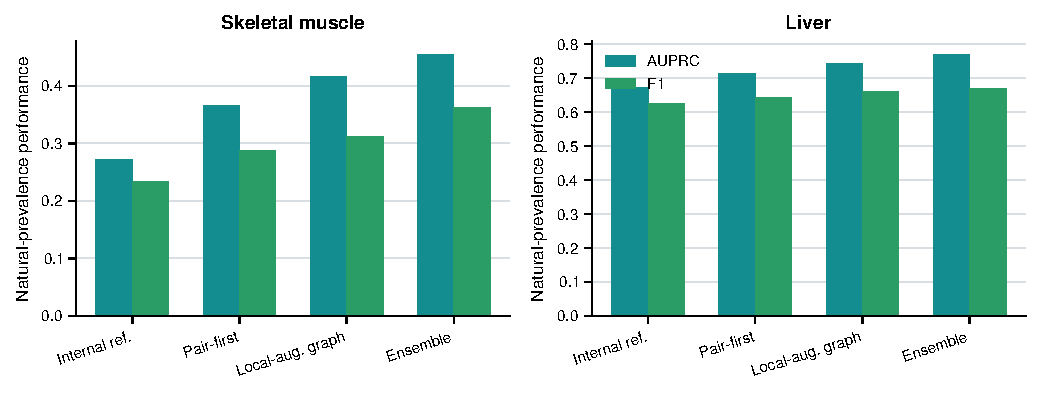
\includegraphics[width=\textwidth]{figures/figureS3_natural_prevalence.pdf}
\caption{\textbf{Secondary natural-prevalence development evaluation.} Performance for the same-fold internal reference, pair-first whole-duplex model, target-local component, and fixed ensemble on all eligible high/low observations from unchanged muscle and liver development pairs.}
\label{fig:s3}
\end{figure}

\begin{table}[H]
\centering
\caption{Secondary natural-prevalence development evaluation. All eligible high/low observations from unchanged development pairs are included; fold-specific validation thresholds are used.}\label{tab:natural}
\resizebox{\textwidth}{!}{%
\begin{tabular}{llrrrrrrr}
\toprule
Context & Model & $n$ & AUROC & AUPRC & F1 & Precision & Recall & FP \\
\midrule
Skeletal muscle & Internal reference & 54289 & 0.8478 & 0.2711 & 0.2328 & 0.1351 & 0.8415 & 15804 \\
Skeletal muscle & Pair-first whole-duplex & 54289 & 0.8900 & 0.3659 & 0.2868 & 0.1714 & 0.8773 & 12441 \\
Skeletal muscle & Local-augmented graph & 54289 & 0.9072 & 0.4166 & 0.3125 & 0.1900 & 0.8800 & 11007 \\
Skeletal muscle & Fixed ensemble & 54289 & 0.9165 & 0.4540 & 0.3621 & 0.2306 & 0.8422 & 8245 \\
Liver & Internal reference & 38096 & 0.8915 & 0.6732 & 0.6246 & 0.4906 & 0.8592 & 6690 \\
Liver & Pair-first whole-duplex & 38096 & 0.9094 & 0.7128 & 0.6418 & 0.5056 & 0.8785 & 6442 \\
Liver & Local-augmented graph & 38096 & 0.9200 & 0.7432 & 0.6602 & 0.5265 & 0.8851 & 5969 \\
Liver & Fixed ensemble & 38096 & 0.9290 & 0.7687 & 0.6684 & 0.5306 & 0.9028 & 5988 \\
\bottomrule
\end{tabular}}
\end{table}


\section*{J. Preregistered unified end-to-end experiment}

After the prediction-level ensemble was frozen but before test access, a separate protocol specified one connected model. A shared three-layer graph attention encoder produced whole-duplex and focal-node states; the aligned local CNN supplied the third view. The three projected representations and their pairwise elementwise interactions entered a 64-unit fusion layer, while a training-only substrate head carried fixed loss weight \UnifiedAuxWeight{}. The connected model had \UnifiedParameters{} trainable parameters versus \EnsembleParameters{} parameters across the two independent ensemble components. Training used pair-first class balance, \UnifiedEpochs{} epochs, Adam at learning rate $10^{-3}$ and weight decay $10^{-4}$, batch size \UnifiedBatchSize{}, and seed \UnifiedBaseSeed{}. The comparator prediction hash and staged decision rules were preregistered.

The unified model's AUROC and AUPRC were below the frozen ensemble in every outer fold (Fig.~\ref{fig:s4}; Table~\ref{tab:unified}). Aggregate F1 was similar, but ranking intervals were entirely adverse and calibration was substantially worse. The conditional no-auxiliary repair, liver replication, and all-context stages were therefore not opened. This preserves the decision rule and shows that independently trained representations were more reliably combined at prediction level than through the tested joint optimization.

\begin{figure}[H]
\centering
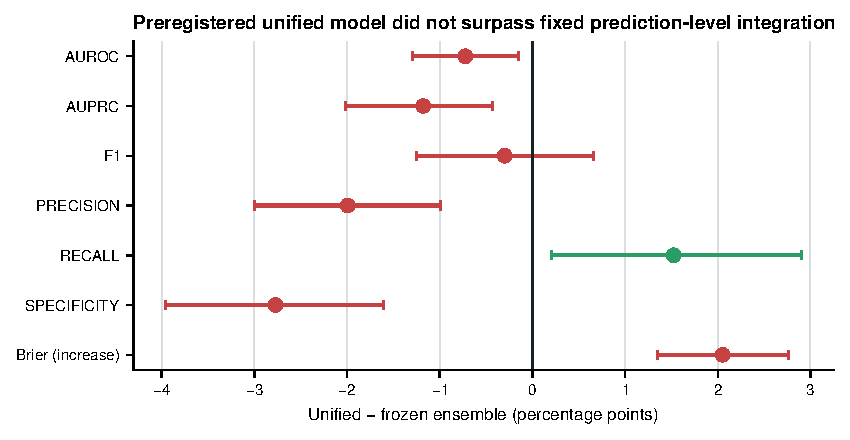
\includegraphics[width=0.84\textwidth]{figures/figureS4_unified_negative_result.pdf}
\caption{\textbf{Preregistered unified model versus the immutable ensemble.} Bars are 95\% whole-pair bootstrap intervals for unified minus ensemble in muscle development OOF data. A positive Brier difference is adverse.}
\label{fig:s4}
\end{figure}

\begin{table}[H]
\centering
\caption{\textbf{The joint model loses ranking and probability accuracy without a clear F1 gain.} In the preregistered skeletal-muscle development comparison, the unified architecture has lower AUROC and AUPRC and higher Brier error than the fixed ensemble. Its higher recall does not compensate on the selection criteria, and the branch stopped before canonical-test access. Pair-clustered intervals give unified-minus-ensemble differences; positive Brier differences are adverse.}\label{tab:unified}
\resizebox{\textwidth}{!}{%
\begin{tabular}{lrrrrrrr}
\toprule
Model & AUROC & AUPRC & F1 & Precision & Recall & Specificity & Brier \\
\midrule
Internal reference & 0.8456 & 0.8256 & 0.7783 & 0.7238 & 0.8415 & 0.6894 & 0.1695 \\
Unified end-to-end & 0.9072 & 0.8922 & 0.8317 & 0.8074 & 0.8575 & 0.8022 & 0.1372 \\
Frozen ensemble & 0.9142 & 0.9040 & 0.8347 & 0.8273 & 0.8422 & 0.8299 & 0.1168 \\
Local-augmented graph & 0.9045 & 0.8936 & 0.8337 & 0.7920 & 0.8800 & 0.7765 & 0.1286 \\
\bottomrule
\end{tabular}}
\vspace{6pt}

\begin{tabular}{lr}
\toprule
Metric & Unified $-$ ensemble, points [95\% CI] \\
\midrule
AUROC & -0.72 [-1.29, -0.15] \\
AUPRC & -1.18 [-2.02, -0.43] \\
F1 & -0.30 [-1.25, +0.66] \\
PRECISION & -1.99 [-3.00, -0.99] \\
RECALL & +1.52 [+0.21, +2.91] \\
SPECIFICITY & -2.77 [-3.96, -1.60] \\
BRIER & +2.05 [+1.35, +2.76] \\
\bottomrule
\end{tabular}
\end{table}


\section*{K. Final training and one-use canonical evaluation}

For each endpoint, pair-first whole-duplex and aligned-local components were fitted on the published training pairs. Published validation data selected checkpoints and one ensemble threshold per endpoint. Ten checkpoints, histories, configurations, selected epochs, thresholds, inputs, code revision, and weights were written to \texttt{provenance/final\_pipeline\_manifest.json}, which retains the exact manifest SHA-256 and bound code revision. The authorization was consumed at 2026-08-25 04:28:30 UTC and records one evaluation. No subsequent model decision used test outcomes.

ADARPro improved ROC and precision--recall curves in every endpoint (Fig.~\ref{fig:s5}); exact performance is in Table~\ref{tab:lockedmetrics}. At frozen thresholds, false-positive rescue exceeded true-positive damage. Matched-recall counts are point estimates obtained by descriptive rethresholding on final predictions; the bootstrap distribution quantifies their pair-clustered uncertainty (Table~\ref{tab:falsepositives}). Reliability curves and lower Brier scores show that ranking gains did not sacrifice calibration (Fig.~\ref{fig:s6}).

\begin{figure}[H]
\centering
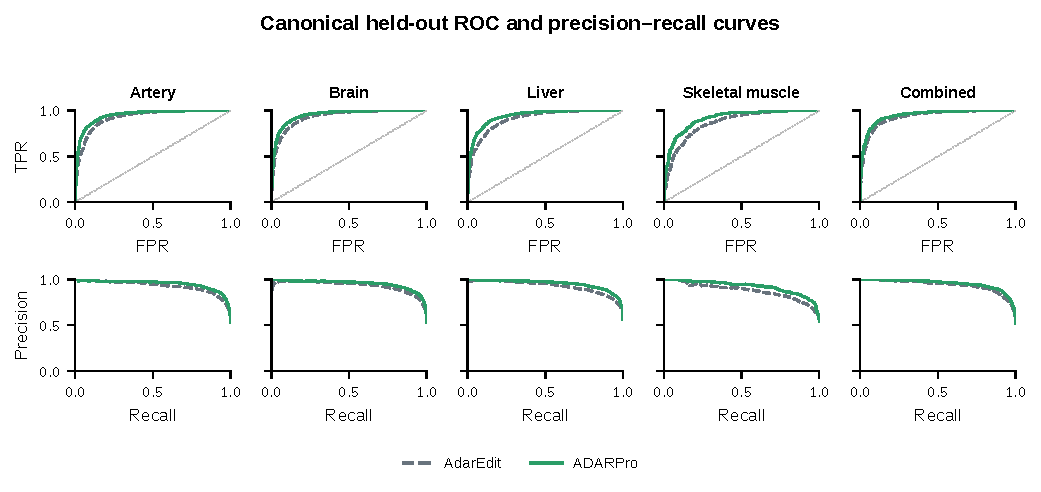
\includegraphics[width=\textwidth]{figures/figureS5_locked_curves.pdf}
\caption{\textbf{Canonical held-out ROC and precision--recall curves.} ADARPro and supplied-checkpoint AdarEdit are shown for four individual tissue endpoints and Combined.}
\label{fig:s5}
\end{figure}

\begin{center}
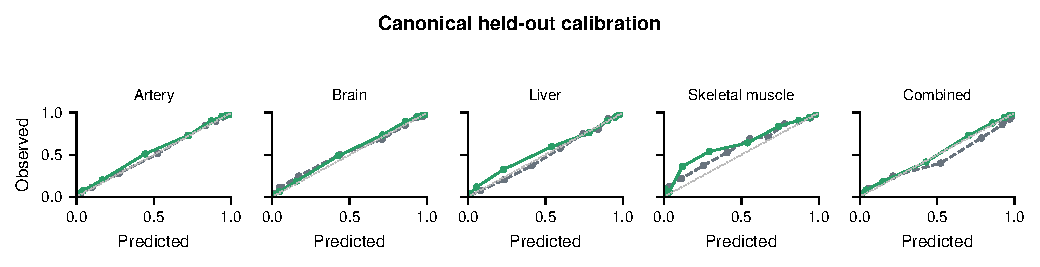
\includegraphics[width=\textwidth]{figures/figureS6_locked_calibration.pdf}
\captionof{figure}{\textbf{Canonical held-out calibration.} Reliability curves for ADARPro and supplied-checkpoint AdarEdit. Brier score is lower for ADARPro in every endpoint.}
\label{fig:s6}
\end{center}

\begin{table}[H]
\centering
\caption{\textbf{False-positive reduction persists at matched recall.} At frozen validation-selected thresholds, rescue and damage percentages use baseline false positives and true positives, respectively; ``New FP'' counts new false positives. The final column matches published-baseline recall exactly. This rethresholding is post-test descriptive, not model selection.}\label{tab:falsepositives}
\resizebox{\textwidth}{!}{%
\begin{tabular}{lrrrrr}
\toprule
Context & Baseline FP & FP corrected (\%) & New FP & TP damaged (\%) & FP avoided at matched recall \\
\midrule
Artery & 460 & 202 (43.9\%) & 42 & 113 (4.9\%) & 126 \\
Brain & 425 & 164 (38.6\%) & 55 & 73 (3.3\%) & 119 \\
Liver & 399 & 202 (50.6\%) & 43 & 121 (5.9\%) & 158 \\
Skeletal muscle & 188 & 83 (44.1\%) & 41 & 28 (4.3\%) & 68 \\
Combined & 459 & 147 (32.0\%) & 116 & 38 (1.7\%) & 148 \\
\bottomrule
\end{tabular}}
\end{table}


\section*{L. Complete campaign taxonomy and provenance}

Table~\ref{tab:taxonomy} records every ranked research direction and its final disposition, including branches deferred for unavailable measurements. The immutable registry at \texttt{experiments/experiments.csv} contains one row per run with code revision, input hashes, fold definition, seed, features, hyperparameters, artifact path, serialized metrics, and test-access status. Exact OOF predictions, fold-level tables, controls, ablations, and bootstrap results remain under \texttt{experiments/runs/}; reports 00--20 preserve chronological interpretation and stopping decisions. A machine-generated numerical claim ledger maps paper quantities to authoritative artifacts and selectors. This repository-level record is more complete and useful than a page of run-family counts.

\begin{longtable}{p{0.06\textwidth}p{0.14\textwidth}p{0.33\textwidth}p{0.37\textwidth}}
\caption{Complete ranked performance-frontier taxonomy and final campaign decision. Full hypotheses, data sources, leakage risks, promotion rules, kill rules, and result summaries are retained in \texttt{experiments/performance\_frontier\_opportunities.csv}.}\label{tab:taxonomy}\\
\toprule
Rank & Axis & Direction & Final disposition \\
\midrule
\endfirsthead
\multicolumn{4}{l}{\textit{Table S7 continued}}\\
\toprule
Rank & Axis & Direction & Final disposition \\
\midrule
\endhead
1 & Biology & IRAlu architecture + transcript state & Broad panel terminated; geometry retained mechanistically \\
1.8 & AI & Expanded high/low supervision & Selected component \\
2 & AI & Continuous + ordinal + binary multi-task & Limited ranking signal; not selected \\
2.2 & Biology $\times$ AI & Expanded cross-tissue shared supervision & Limited shared signal; not selected \\
2.5 & Biology $\times$ AI & Cross-fitted all-adenosine substrate profile & Terminated after stronger-model control \\
3 & Biology $\times$ AI & Substrate-wide multi-A + engagement latent & Terminated in tested formulation \\
3.4 & Biology $\times$ AI & Target-centered ADAR contact geometry & Advanced to aligned local encoder \\
3.45 & AI & Focal-node + global graph pooling & Validated fallback/complementary view \\
3.5 & AI & Target-local multiscale CNN + graph fusion & Selected component \\
4 & Biology & Chromatin/co-transcriptional state & Bulk peak-overlap formulation terminated \\
5 & Biology $\times$ AI & Hierarchical engagement $\times$ site chemistry & Stopped for futility \\
6 & Biology & In-vivo/ensemble RNA structure & Deferred: coverage/context mismatch \\
7 & Biology $\times$ AI & Donor/sample-level multimodal model & Deferred: no matched donor outcomes \\
7.5 & AI & Self-supervised IRAlu pretraining & Deferred: corpus not benchmark-ready \\
8 & AI & Frozen RNA foundation-model fusion & Terminated after 150M-model confirmation \\
8.5 & AI & Graph Transformer / GATv2 multi-scale encoder & Deferred after lower-cost local gain \\
9 & Biology & ADAR isoform/IFN/localization state & Deferred: no matched state/outcomes \\
10 & Biology & Cell-matched perturbation RBP effects & Deprioritized after RBP branch \\
11 & AI & Calibration/stacking/ensemble & Selected final integration \\
11.5 & AI $\times$ Biology & Unified end-to-end representation learning & Terminated after preregistered primary \\
12 & AI & Larger/deeper GNN alone & Terminated \\
13 & Biology & Generic RBP binding $\times$ bulk GTEx & Terminated \\
\bottomrule
\end{longtable}


\section*{M. Interpretation and decisive future measurements}

The evidence supports three biological levels and one learning principle. Whole-duplex sequence and structure encode intrinsic competence. Pair geometry and editing burden demonstrate a substrate-realization state, but current bulk context features cannot estimate its realized cellular value. Target/partner alignment recovers local selectivity. Pair-first sampling respects the dependence among observations from one duplex. The selected predictor integrates the two actionable representations without claiming to measure cellular environment directly.

The next high-information study should pair donor- or cell-resolved editing with transcript abundance, splicing and intron retention, ADAR1 isoform and interferon state, regulator activity, quantitative chromatin, and in-vivo RNA structure from the same samples. Perturbing ILF2/ILF3/ZFR-family regulators on substrates selected for high intrinsic competence would distinguish occupancy correlation from causal suppression. Such measurements could finally test a two-stage model in which cellular state controls substrate realization and local RNA context controls adenosine selectivity.

\FloatBarrier
\bibliography{references}

\end{document}
